\documentclass[11pt]{article}
\usepackage[a4paper,margin=23mm]{geometry}
\usepackage{graphicx,booktabs,longtable}
\title{NoLA on EuroSAT: a small case study}
\date{}
\begin{document}
\maketitle
\section{Design and provenance}
Selected GPU validation run: NoLA 141/240, CDE 117/240, DINO head 134/240. The tables below are a separate CPU replay, not the original GPU measurements. Data: 160 adaptation, 240 validation, and a 240-image fixed test audit excluding the 80 earlier teaching test images. The recipe was selected on validation, not on this test audit.
\begin{itemize}
\item train\_n: 160
\item anchor\_cap: 4
\item head\_batch: 8
\item head\_epochs: 3
\item prompts: 16
\item clip\_batch: 4
\item clip\_lr: 0.004
\end{itemize}
\section{Replay results}
\begin{tabular}{lll}\toprule Stage & Validation & Fresh test\\\midrule
Unprompted CLIP CDE & 117/240 (48.75\%) & 130/240 (54.17\%)\\
Fitted DINO head & 134/240 (55.83\%) & 137/240 (57.08\%)\\
Prompted CLIP before training & 41/240 (17.08\%) & 39/240 (16.25\%)\\
Prompted CLIP, epoch 1 & 87/240 (36.25\%) & 74/240 (30.83\%)\\
Prompted CLIP, epoch 4 & 124/240 (51.67\%) & 121/240 (50.42\%)\\
\bottomrule\end{tabular}
\clearpage
\noindent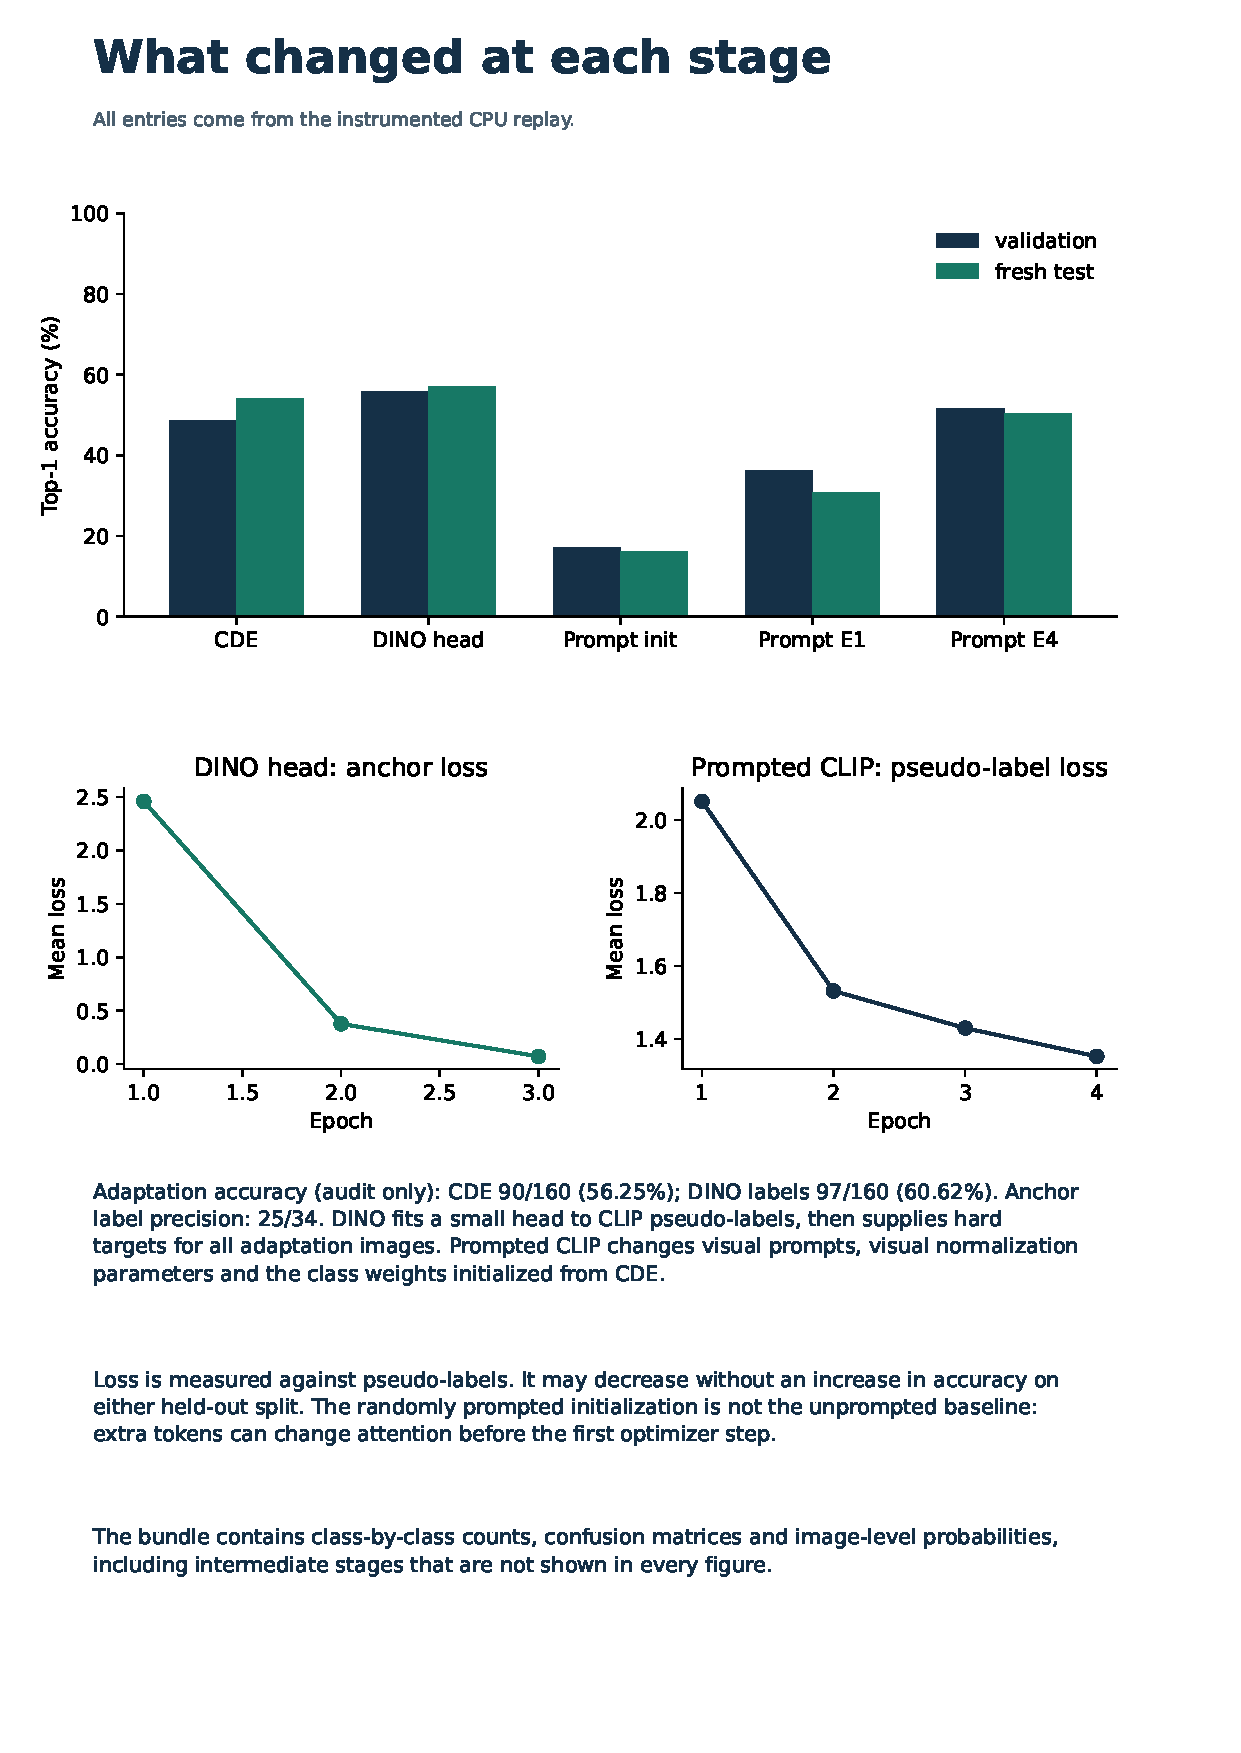
\includegraphics[width=\textwidth,height=0.93\textheight,keepaspectratio]{figures/stage-results.pdf}\clearpage
\noindent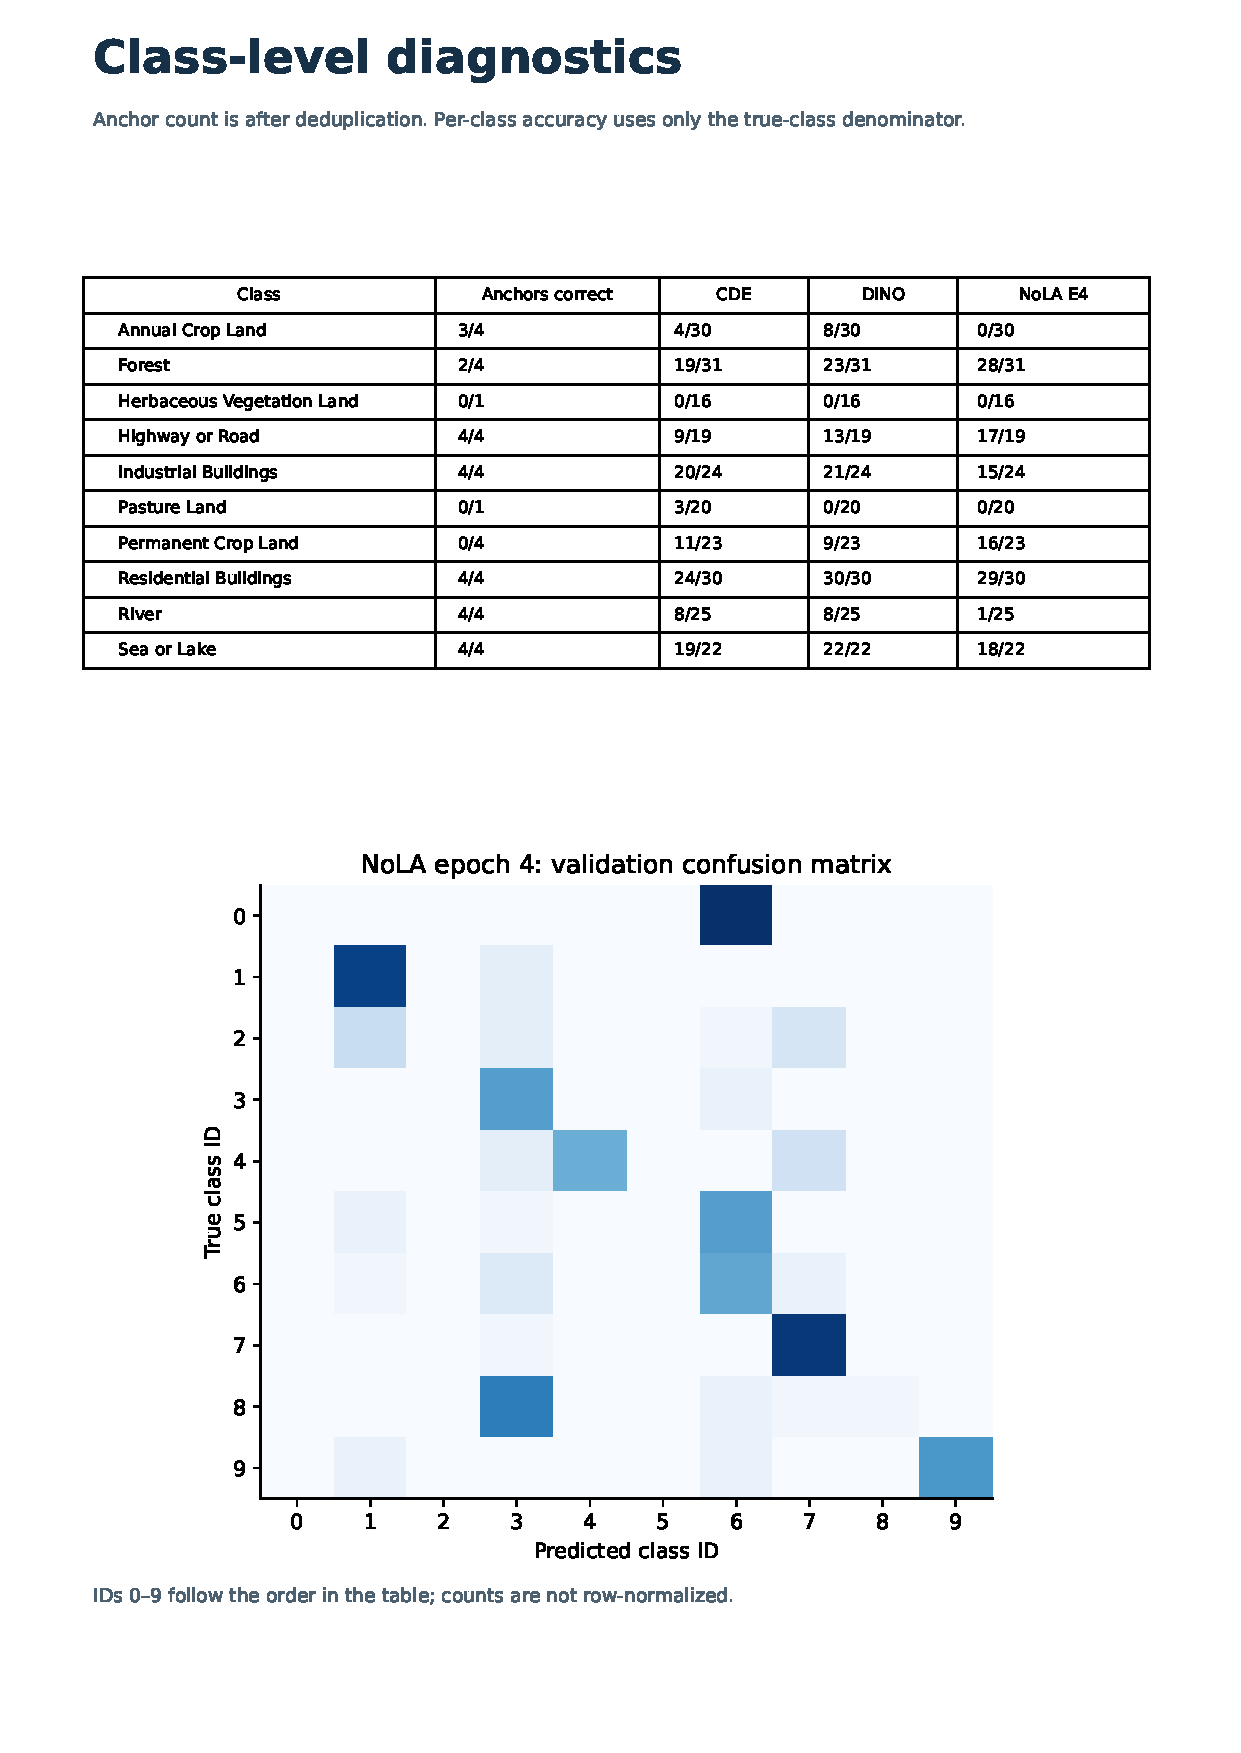
\includegraphics[width=\textwidth,height=0.93\textheight,keepaspectratio]{figures/per-class.pdf}\clearpage
\noindent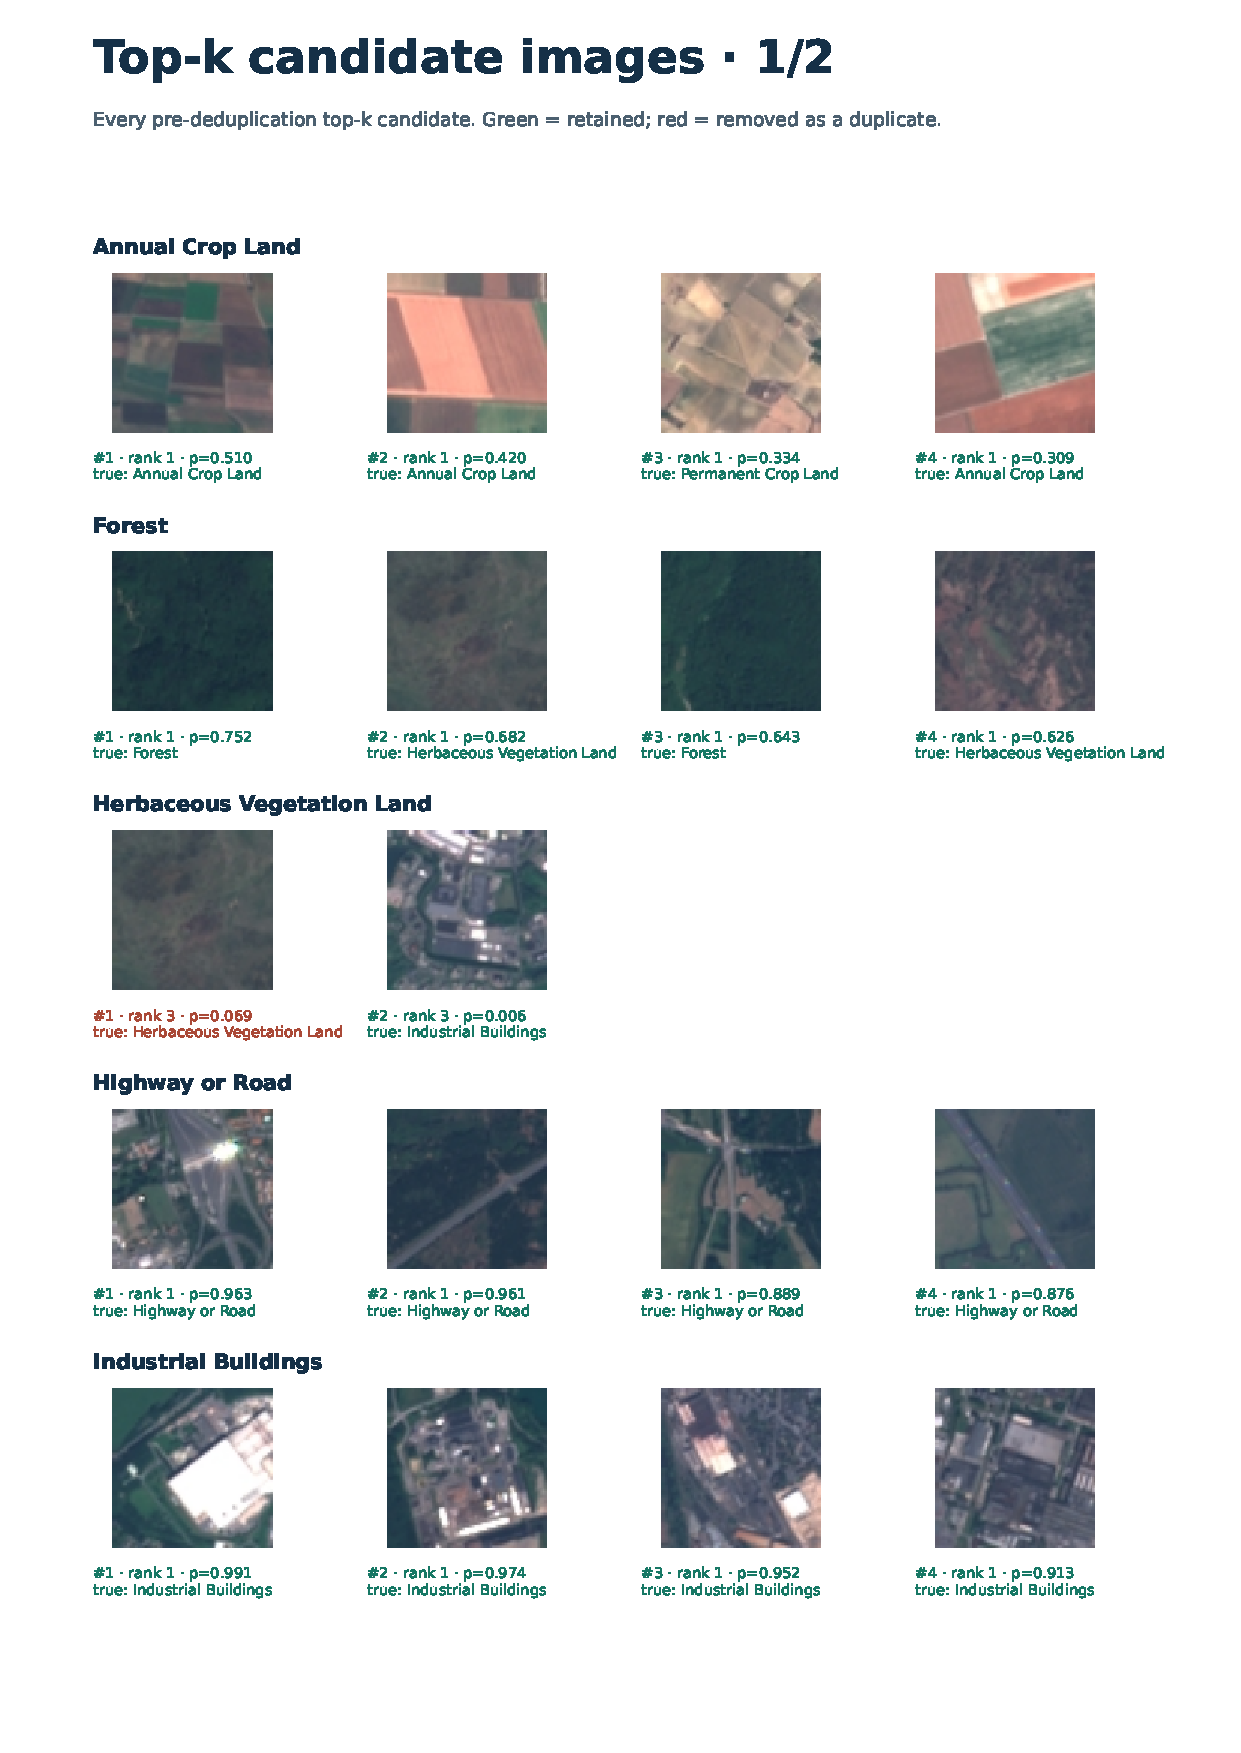
\includegraphics[width=\textwidth,height=0.93\textheight,keepaspectratio]{figures/anchors-1.pdf}\clearpage
\noindent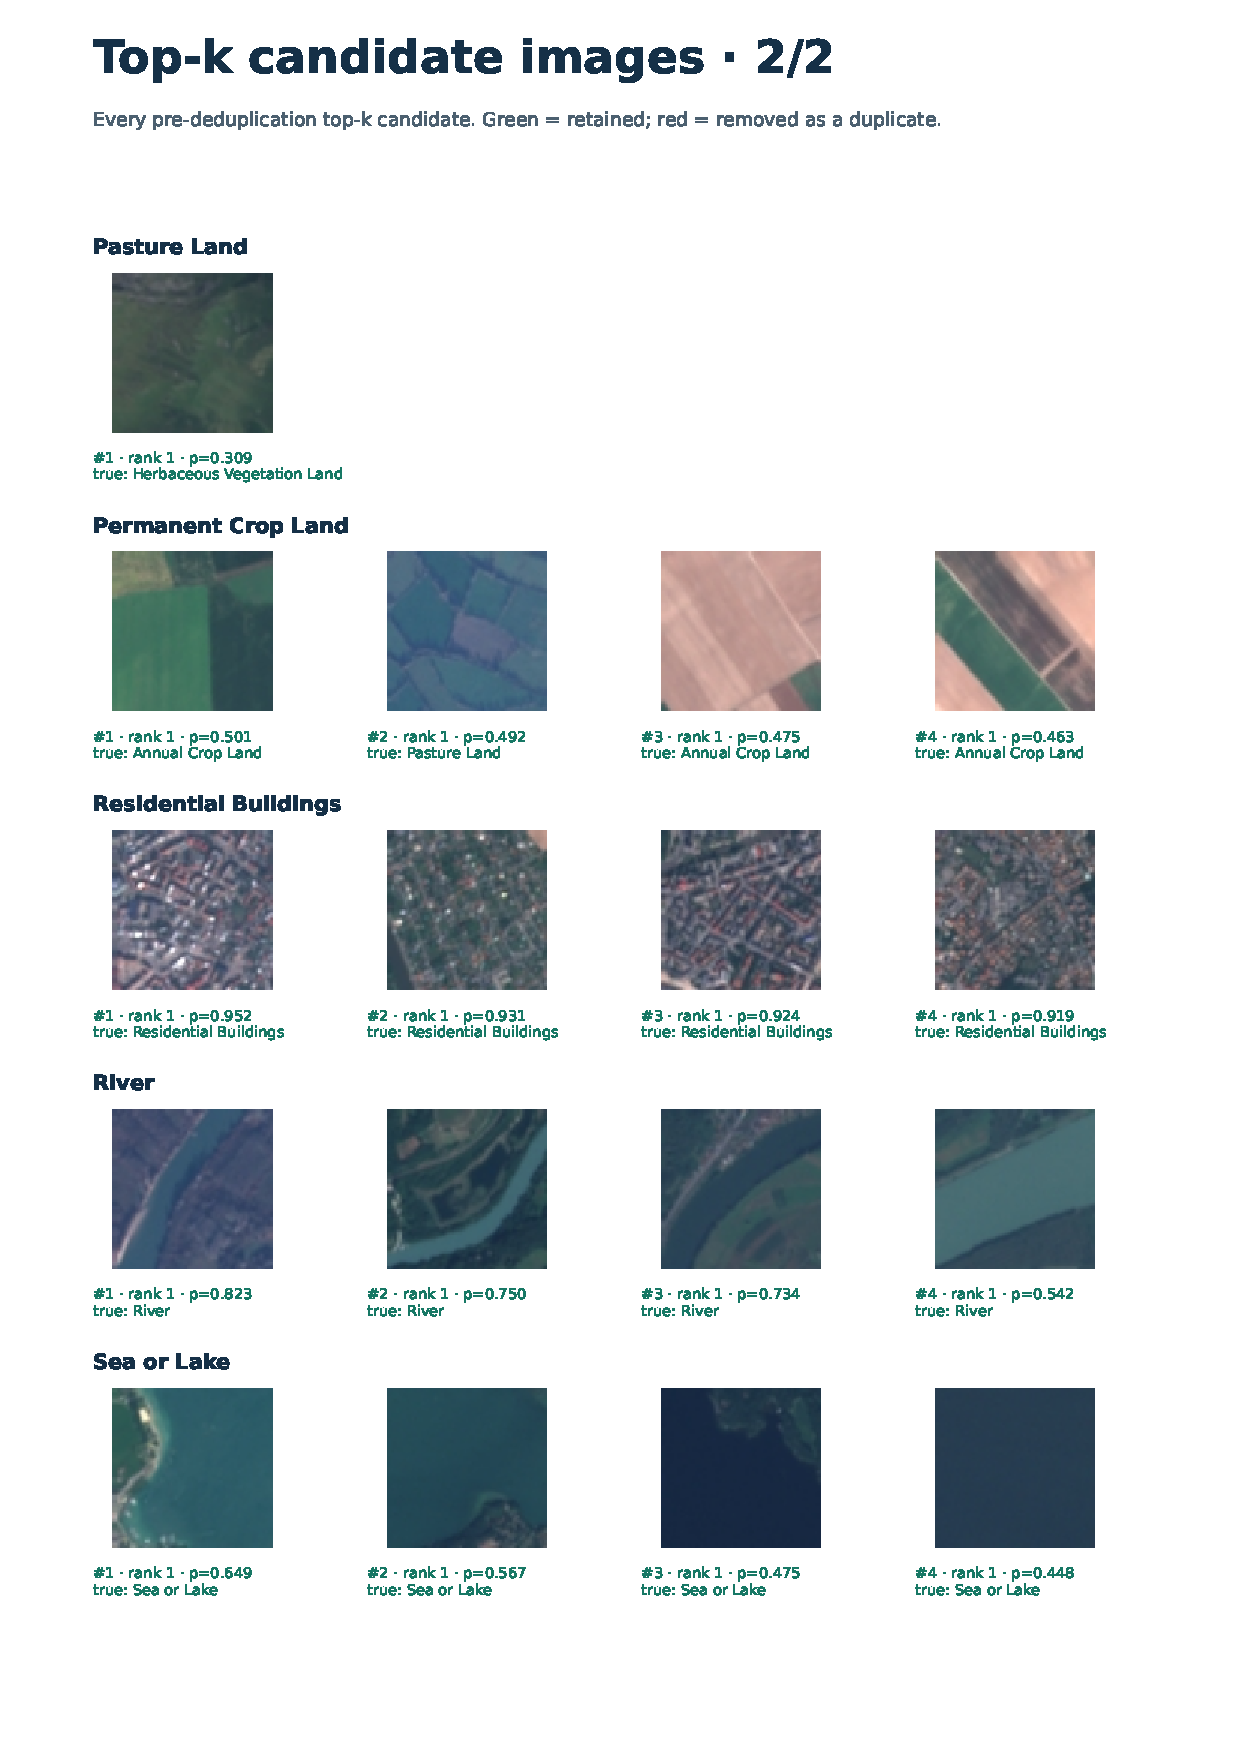
\includegraphics[width=\textwidth,height=0.93\textheight,keepaspectratio]{figures/anchors-2.pdf}\clearpage
\noindent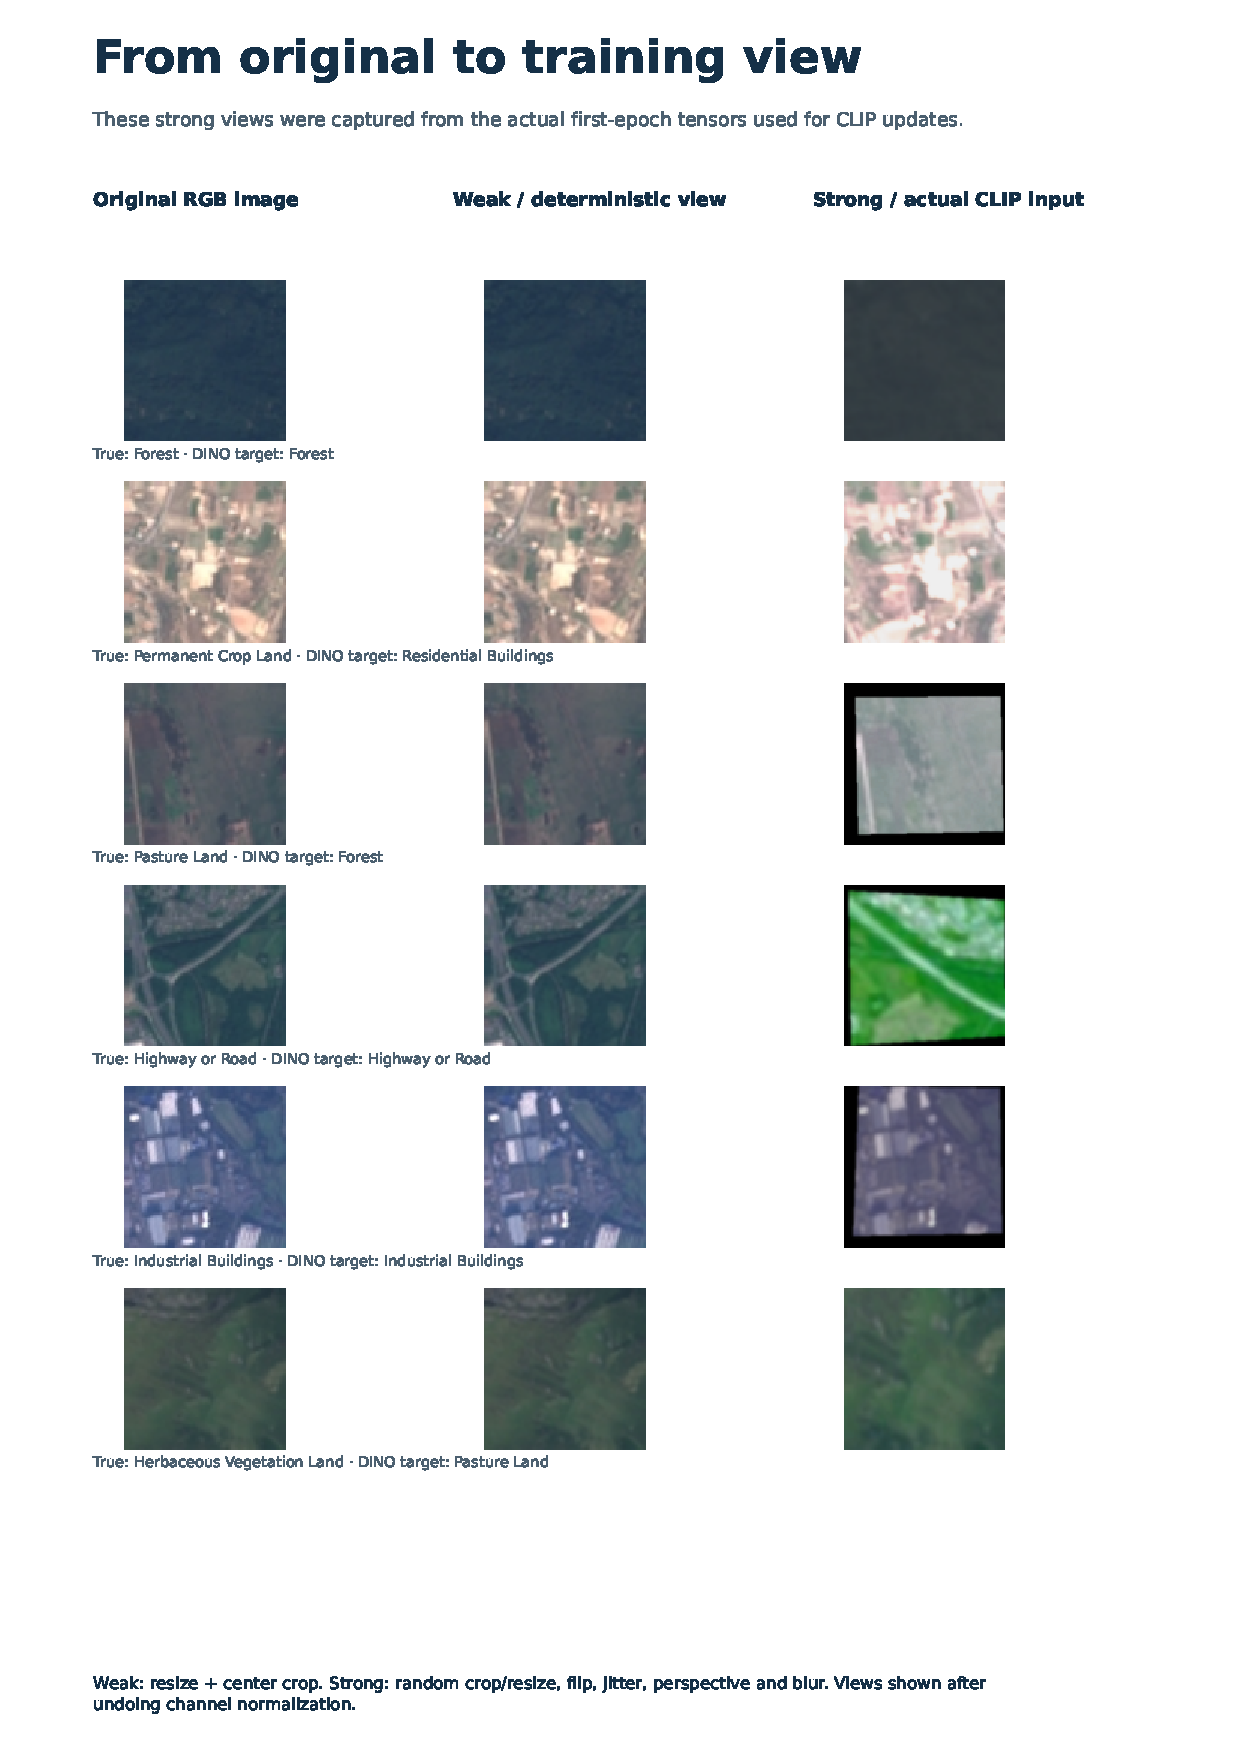
\includegraphics[width=\textwidth,height=0.93\textheight,keepaspectratio]{figures/augmentations.pdf}\clearpage
\noindent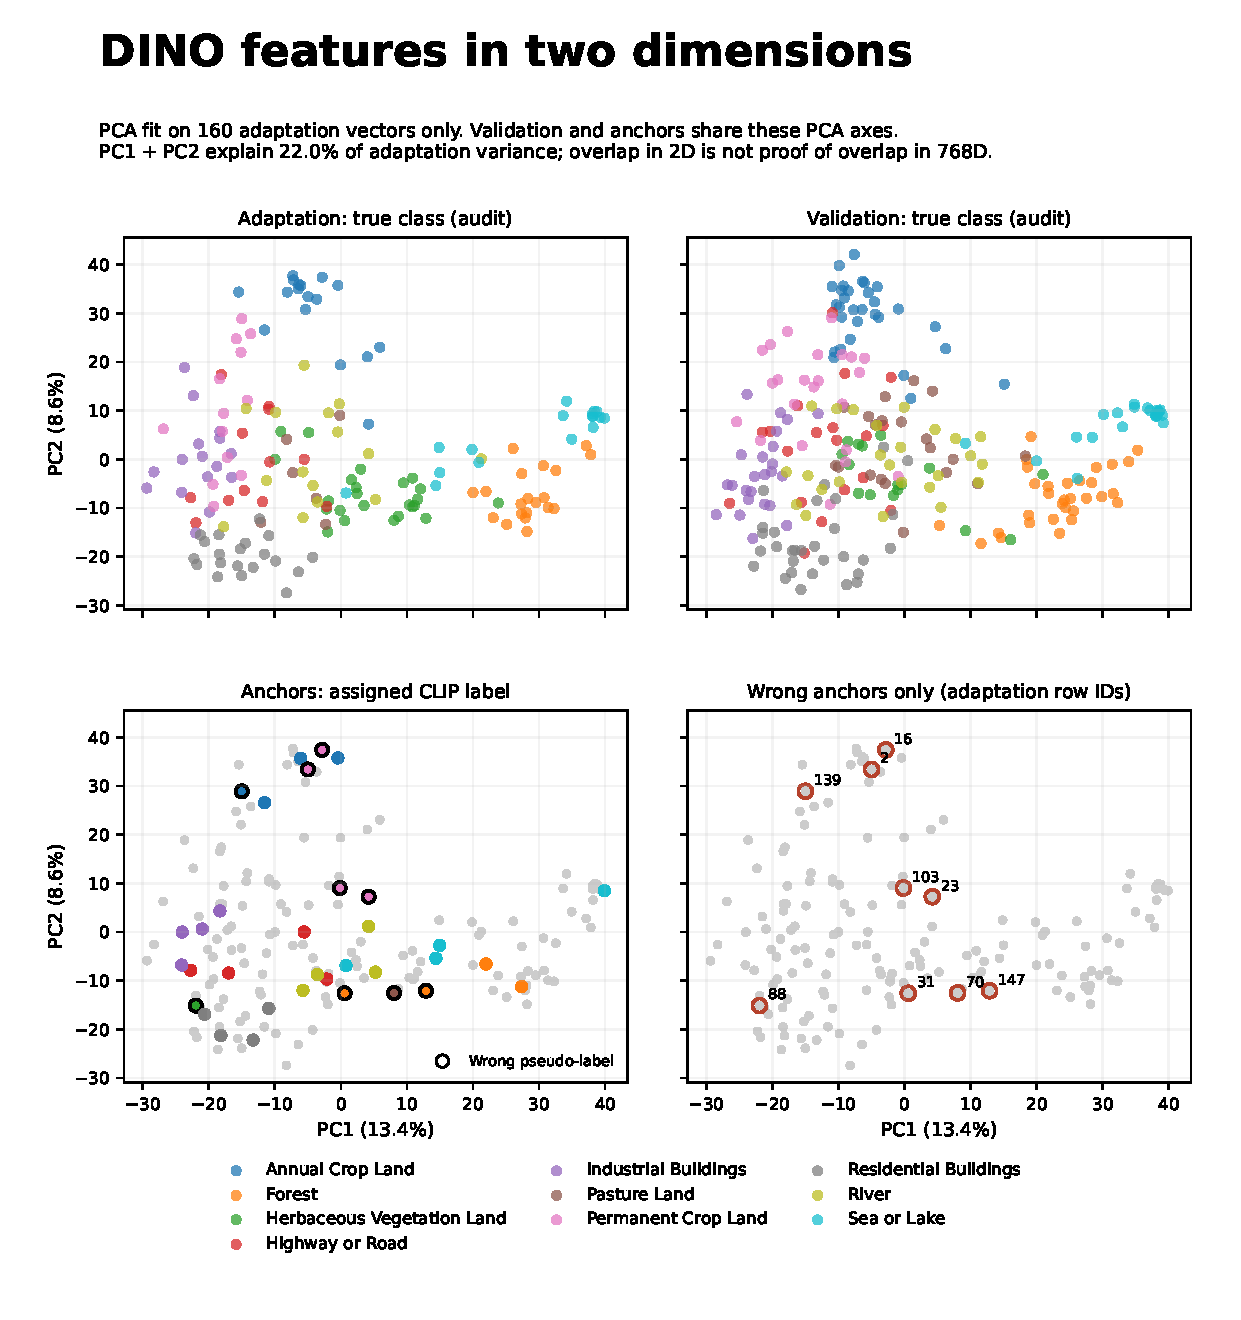
\includegraphics[width=\textwidth,height=0.93\textheight,keepaspectratio]{figures/dino-pca.pdf}\clearpage
\appendix\section{Exact CDE inputs}
\subsection{Annual Crop Land}
\begin{enumerate}
\item A satellite photo of Annual Crop Land will appear as a patchwork quilt of various shades of pale green, brown and yellow.
\item A satellite photo of Annual Crop Land typically looks like a patchwork quilt of various colors.
\item A satellite photo of Annual Crop Land typically looks like a patchwork of green and brown fields.
\item A satellite photo of Annual Crop Land typically appears as a patchwork quilt of earth tones.
\item A satellite photo of Annual Crop Land typically looks like a patchwork quilt, with different colors and shapes showing different crop types.
\item Annual crop land can typically be recognized in satellite photos by the regular geometry of the fields, as well as the bright green color of the vegetation.
\item Satellite photos of annual crop land can usually be recognized by their distinctive rectangular patterns.
\item Annual crop land can be identified in satellite photos by looking for patterns of regular geometric lines in agricultural areas.
\item Annual Crop Land is recognizable on satellite images by its distinct landscape pattern consisting of alternating bands of cultivated fields and non-cultivated areas.
\item Annual Crop Land can be easily recognized in a satellite photo by its rolling or patchwork pattern of cultivated fields, which cover large areas and may be the same crop type or a mosaic of different crops.
\item A satellite photo of annual crop land will typically show a patchwork of different fields containing various types of agricultural crops.
\item A satellite photo of Annual Crop Land typically looks like a patchwork quilt, showing a variety of colors and textures depending on the type of crop being grown.
\item A satellite photo of annual crop land will typically show strips of land with various shades of green.
\item The satellite photo of Annual Crop Land depends on the region, but it typically shows a landscape of fields, plots, and other land that is used for growing crops.
\item Satellite photos of annual crop land will typically show large stretches of land that are either a single color, like a uniform green or tan, or multiple colors ? like the bright yellow of ripening wheat or the dark green of recently planted fields.
\item The satellite photo from the internet of Annual Crop Land shows some remarkable geographical features.
\item The satellite photo of Annual Crop Land from the internet is a high-resolution image that shows the vastness of the land dedicated to agricultural production.
\item The satellite photo from the internet of Annual Crop Land shows a variety of plants and crops growing in an agricultural area.
\item The satellite photo from the internet of Annual Crop Land shows a wide swath of land covered in cultivated crops, typically planted and farmed in a single growing season.
\item The satellite photo from the internet of Annual Crop Land shows an agricultural area with a wide variety of crops planted in neat rows or patches.
\item The satellite photo of Annual Crop Land can be identified by its distinctive pattern.
\item Annual crop land can be identified in a satellite photo by looking for patterns of vegetation such as rows or patches of green, brown, and/or yellow fields.
\item You can identify annual crop land in a satellite photo by looking for distinct patterns, such as rows, circles, or other geometric shapes, that indicate areas devoted to planting and harvesting crops.
\item The most obvious way to identify a satellite photo of Annual Crop Land is to look for rows of planted crops.
\item Satellite images of annual crop lands can be identified by looking for patterns of uniformity in the vegetation coverage within the area.
\end{enumerate}
\paragraph{Filled CLIP templates}\begin{itemize}
\item a satellite photo of Annual Crop Land.
\item a satellite photo of a Annual Crop Land.
\item a satellite photo of the Annual Crop Land.
\item a centered satellite photo of Annual Crop Land.
\item This is an aerial image of a Annual Crop Land.
\item a aerial image of Annual Crop Land.
\end{itemize}
\subsection{Forest}
\begin{enumerate}
\item The satellite photo of the forest is likely to show a patchwork of varying shades of green.
\item A satellite photo of a forest typically looks like a patchwork quilt of green, with patches of lighter green or yellow, indicative of trees, shrubs, and other vegetation growing in the area.
\item The satellite photo of the forest would show trees and vegetation in green, with the darker shades of green representing denser trees and canopy coverage.
\item A satellite photo of a forest looks like a patchwork quilt of varying shades of green.
\item The satellite photo of a forest usually looks like a mix of green and brown patches.
\item To recognize a satellite photo of a forest, look for a geographic area with large patches of green vegetation and other features associated with forests, such as wetlands, streams, rivers, and lakes.
\item The most obvious way to recognize a satellite photo of a forest is to look for large clusters of trees.
\item One way to recognize a satellite photo of a forest is to look for a pattern of trees arranged in a linear or rectangular shape.
\item Satellite photos of forests are typically characterized by a patchwork of green areas, often with areas of bare ground, and roads, rivers, and other infrastructure networks.
\item The satellite photo of a forest can be recognized by its pattern of trees and the amount of greenery that can be seen.
\item The satellite photo of Forest shows a densely wooded area with a mix of deciduous and evergreen trees.
\item A satellite photo of a forest will typically look like a lush green mass of trees with patches of land visible between them.
\item A satellite photo of a forest will likely show a pattern of trees and various shades of green to depict the canopy.
\item A satellite photo of a forest would likely show a large, green area with various types of trees.
\item The satellite photo of Forest is a bird's-eye view of the town and its surrounding environment.
\item The satellite photo of the forest on the internet most likely shows a patch of natural land covered in varying degrees of greenery.
\item The satellite photo from the internet of the forest shows a vast expanse of green trees and foliage.
\item This satellite photo of a forest shows a large expanse of lush green trees in an area of rolling hills.
\item This satellite photo shows an expanse of forested land.
\item The satellite photo from the internet is of a dense forest located in a mountainous region.
\item If you know the geographic area or location, you can use satellite mapping services like Google Earth or Google Maps to identify the satellite photo of the forest.
\item
You can identify the satellite photo of a forest by its distinct features such as tree canopy cover, patterns of the forest, and ground features like streams visible on the ground.
\item The most reliable way to identify a satellite photo of forest is by looking for specific features.
\item To identify the satellite photo of a forest, you can look for the tell-tale signs of trees, which typically appear as a blanket of green in satellite images.
\item There are a few different ways to identify a satellite photo of a forest, such as using satellite imagery and ground references.
\end{enumerate}
\paragraph{Filled CLIP templates}\begin{itemize}
\item a satellite photo of Forest.
\item a satellite photo of a Forest.
\item a satellite photo of the Forest.
\item a centered satellite photo of Forest.
\item This is an aerial image of a Forest.
\item a aerial image of Forest.
\end{itemize}
\subsection{Herbaceous Vegetation Land}
\begin{enumerate}
\item A satellite photo of Herbaceous Vegetation Land will typically appear in shades of green, indicating the presence of foliage or grasses.
\item The satellite photo of Herbaceous Vegetation Land will typically feature an array of green hues that vary in intensity.
\item A satellite photo of herbaceous vegetation land typically looks lush and green.
\item A satellite photo of Herbaceous Vegetation Land typically shows an area with low growing, herbaceous plants, such as grasses, wildflowers, sedges, and forbs.
\item The satellite photo of Herbaceous Vegetation Land usually looks like a patchwork of green and brown.
\item Herbaceous vegetation usually appears light green in satellite images due to the presence of chlorophyll in the small leaves and stems.
\item Herbaceous vegetation land can be identified in a satellite photo by its bright green color and more uniform texture compared to other vegetation types.
\item Herbaceous vegetation land can be identified in a satellite photo by the presence of green vegetation and soil with minimal foliage or trees.
\item Herbaceous vegetation land can be recognized in satellite images by looking for large areas of green and patches of lighter green and yellow, which indicate healthy vegetation.
\item The satellite photo of Herbaceous Vegetation Land will likely contain a lot of green, as the vegetation is composed of grasses, herbs, forbs, and other non-woody plants.
\item A satellite photo of Herbaceous Vegetation Land will show a large area of green space, dominated by grasses, herbs, annuals, and perennials.
\item Herbaceous vegetation land is typically characterized by lush green vegetation, including grasses, flowers, weeds, and other low-growing plants.
\item Satellite photos of herbaceous vegetation land can vary widely depending on the type of vegetation present.
\item A satellite photo of herbaceous vegetation land typically shows a range of colors from various greens and yellows.
\item A satellite photo of herbaceous vegetation land typically looks like an image of bright greens, yellows, and other colors of vegetation.
\item This satellite photo depicts Herbaceous Vegetation Land, which is defined by a type of vegetation that consists mainly of flowering plants and grasses.
\item The satellite photo from the internet of Herbaceous Vegetation Land shows a large expanse of mostly green vegetation, with some small patches of bare ground.
\item The satellite photo from the internet of Herbaceous Vegetation Land is a picture of green land that shows a variety of different shapes and sizes of vegetation.
\item The satellite photo from the internet of Herbaceous Vegetation Land is a detailed, high-resolution image of the landscape from an aerial perspective.
\item The satellite photo from the internet of Herbaceous Vegetation Land shows an area of treeless vegetation, primarily with grass and other low-growing non-woody plants.
\item Identifying herbaceous vegetation land from satellite photos is generally done by looking for patterns and clusters of vegetation that typical of the life form.
\item To identify a satellite photo of Herbaceous Vegetation Land, you should look for clouds and water, prominent plants with flat leaf blades, and soils.
\item By identifying the features typical of herbaceous vegetation land, such as the different shades of green and the absence of trees, it is possible to identify a satellite photo of herbaceous vegetation land.
\item The satellite photo of Herbaceous Vegetation Land can be identified by looking for a combination of variations in color or texture in the image.
\item The satellite photo of Herbaceous Vegetation Land can be identified by its distinct characteristics which include a high amount of green color from grasses, shrubs, and herbs, flecks of trees, and sparse patches of bare soil.
\end{enumerate}
\paragraph{Filled CLIP templates}\begin{itemize}
\item a satellite photo of Herbaceous Vegetation Land.
\item a satellite photo of a Herbaceous Vegetation Land.
\item a satellite photo of the Herbaceous Vegetation Land.
\item a centered satellite photo of Herbaceous Vegetation Land.
\item This is an aerial image of a Herbaceous Vegetation Land.
\item a aerial image of Herbaceous Vegetation Land.
\end{itemize}
\subsection{Highway or Road}
\begin{enumerate}
\item A satellite photo of a highway or road typically includes a large asphalt or dirt strip with other nearby roads.
\item A satellite photo of a highway or road typically shows a wide network of paved lanes and access roads, with cars visible as small, white dots zooming across.
\item A satellite photo of a highway or road will usually show a clear image of the lanes, side streets, and exits on the highway.
\item Satellite photos of highways and roads typically feature a wide aerial view of the route.
\item A satellite photo of a highway or road typically shows a wide, straight ribbon of asphalt winding through the landscape.
\item Satellite photos of highways or roads can be recognized by looking for straight lines with consistent width or features such as turn-offs, bridges, cloverleafs, or exits.
\item Satellite photos of highways and roads can be recognized by the distinct straight lines, with regularly spaced intersections, that typically form a web-like pattern.
\item The easiest way to recognize a satellite photo of a highway or road is to look for the straight lines and smooth curves that are common in road designs.
\item Satellite photos of highways and roads can be identified by finding long, straight, linear features in the image, as well as other road features such as highways interchanges, bridges, tunnels, and exit and entrance ramps.
\item Satellite photos of highways or roads can be easily recognized by the linear shapes and straight lines that denote the various lanes, intersections, and entrance/exit points, as well as the many various features that are associated with roads such as road signs.
\item A satellite photo of a highway or road may show a wide stretch of asphalt that appears gray or black against the surrounding area.
\item A satellite photo of a highway or road will typically include a wide swath of asphalt or concrete running through the landscape, as well as any nearby buildings, homes, trees, and other features of the landscape.
\item A satellite photo of a highway or road typically appears as an aerial view of the highway, usually consisting of a two-lane stretch with small white stripes defining each lane and surrounding the highway.
\item A satellite photo of a highway or road would typically show the entire stretch of the highway or road as a ribbony line running through a landscape or within a cityscape.
\item A satellite photo of a highway or road will usually show the wide expanse of the roadway, with multiple lanes of traffic in either direction and multiple off-ramps and side roads branching off from the main highway.
\item The satellite photo from the internet of a highway or road is a high-resolution image provided by an overhead satellite.
\item The satellite photo from the internet of a highway or road shows a bird's-eye view of the route.
\item The satellite photo from the internet of a highway or road typically shows a curvy road cutting through a rural or urban environment with buildings, trees, and other landmarks visible in the background.
\item The satellite photo from the internet of a highway or road is a high resolution image that allows viewers to see the details of the landscape and the layout of the road.
\item A satellite photo of a highway or road is an aerial view of the road taken from a satellite's point of view.
\item To identify a satellite photo of a highway or road, look for long, straight lines that indicate a man-made structure.
\item To identify a satellite photo of a highway or road, look for distinguishing features such as a straight line or multiple lanes of traffic.
\item
The easiest way to identify a satellite photo of a highway or road is to look for the distinct lines and curves of pavement which are generally much wider than a typical street.
\item Satellite photos of roads and highways can usually be identified by the straight lines created by the outlines of the road, as well as the shadows created by overhead structures, such as bridges or overpasses.
\item To identify the satellite photo of a highway or road, look for the distinct features found in typical roadways, such as long straight lines and regular intersections of intersecting roads.
\end{enumerate}
\paragraph{Filled CLIP templates}\begin{itemize}
\item a satellite photo of Highway or Road.
\item a satellite photo of a Highway or Road.
\item a satellite photo of the Highway or Road.
\item a centered satellite photo of Highway or Road.
\item This is an aerial image of a Highway or Road.
\item a aerial image of Highway or Road.
\end{itemize}
\subsection{Industrial Buildings}
\begin{enumerate}
\item A satellite photo of industrial buildings might look like a patchwork of utilitarian structures.
\item Satellite photos of industrial buildings typically show a large complex of buildings and structures, highlighted by their distinctive shapes and offsets.
\item A satellite photo of industrial buildings would typically show large rows of buildings with a uniform, rectangular shape.
\item A satellite photo of industrial buildings typically looks like a bird's eye view of an urban area, with a large cluster of buildings spread out across the landscape.
\item A satellite photo of industrial buildings would generally depict a mix of large industrial structures, such as warehouses, manufacturing plants, and storage facilities, as well as smaller buildings that may be part of the complex.
\item Industrial buildings can typically be recognized in satellite photos by their large, flat rooftops and large walls that are designed to facilitate ventilation and provide structural support.
\item Satellite photos of industrial buildings can be identified by the large industrial buildings and equipment such as factories, smokestacks, power plants, oil refineries, and chemical plants.
\item Industrial buildings can be identified in satellite photos by looking for tall structures, smoke or dust clouds, and surrounding asphalt or metal roads.
\item Industrial buildings can often be identified in satellite photos by their distinct shapes and sizes and the presence of large parking lots or storage yards.
\item Industrial buildings in satellite photos can generally be identified by their large, rectangular shapes and uniform patterns of structures and infrastructure.
\item A satellite photo of industrial buildings can vary depending on the area it was shot from.
\item A satellite photo of industrial buildings typically includes a bird's-eye view of a factory, warehouse, or other commercial industrial building.
\item A satellite photo of industrial buildings may look like a series of large, rectangular buildings surrounded by parking lots, roads, and other industrial structures such as manufacturing equipment.
\item Satellite photos of industrial buildings typically show a large, rectangular or cube-like structure with many different levels.
\item Satellite photos of industrial buildings will typically show a large area including a number of buildings, usually of a similar size and shape.
\item The satellite photo from the internet of industrial buildings is an aerial view of a large complex of industrial warehouses, factories and other facilities.
\item The satellite photo of industrial buildings shows a large area filled with commercial and industrial structures.
\item The satellite photo from the internet of industrial buildings shows a close-up view of a group of buildings in an industrial area of a city.
\item The satellite photo from the internet of industrial buildings is a high-res image of a cluster of industrial buildings from an aerial perspective.
\item The satellite photo from the internet of industrial buildings shows a collection of large, rectangular buildings surrounded by a number of smaller structures.
\item To identify the satellite photo of industrial buildings, you can look for tell-tale signs such as large structures with multiple levels, conveyor belts, smokestacks, and other infrastructure associated with manufacturing and production.
\item To identify the satellite photo of Industrial Buildings, look for clues such as rows of large buildings, warehouses, and storage tanks; highways, railroads, or large paved areas; and water or power lines and pipes.
\item 1.
\item You can identify a satellite photo of industrial buildings by looking for certain features.
\item Industrial buildings can be identified in satellite photos by their large size and square or rectangular shapes.
\end{enumerate}
\paragraph{Filled CLIP templates}\begin{itemize}
\item a satellite photo of Industrial Buildings.
\item a satellite photo of a Industrial Buildings.
\item a satellite photo of the Industrial Buildings.
\item a centered satellite photo of Industrial Buildings.
\item This is an aerial image of a Industrial Buildings.
\item a aerial image of Industrial Buildings.
\end{itemize}
\subsection{Pasture Land}
\begin{enumerate}
\item A satellite photo of pasture land typically looks like a patchwork of green grassy fields with little patches of trees, bushes, or hedgerows in between.
\item A satellite photo of pasture land typically includes a wide area of green grass, dotted with trees, shrubs, and other vegetation.
\item A satellite photo of pasture land typically looks like a photo of large green fields interrupted by tree lines, small rivers/streams, and winding pathways.
\item A satellite photo of pasture land typically will show distinct patches of land, often with different shades of green.
\item Satellite photos of pasture land typically appear mostly green, with different shades and textures indicating the type of vegetation present.
\item Satellite photos of pasture land can be identified by looking for large areas of grass or hay fields, orchards, meadows, wetlands, and crop fields bordered by roads and streams.
\item Satellite photos of pasture land can be recognized by looking for squares or rectangles of different shades of green, which are often divided by darker lines that create the boundaries of the pasture land.
\item Satellite photos of pasture land can be identified by looking for areas of land with long, thin rows of vegetation growing in lines, typically spread in a grid pattern.
\item Satellite photos of pasture land are typically characterized by sections of green land divided by roads or streams.
\item Satellite images of pasture land often appear as large green patches with distinct geometric patterns.
\item A satellite photo of a pasture usually shows a large area of lightly to medium-green grass with sporadic trees and other shrubs scattered throughout the area.
\item The satellite photo of pasture land typically looks like a large, flat expanse with a lot of green vegetation.
\item Satellite photos of pasture land typically show large swaths of green, representing the grassy vegetation, as well as the surrounding natural terrain.
\item A satellite photo of pasture land typically features green fields dotted with patches of trees, shrubs, and other vegetation, interspersed with dirt roads, streams, and ponds.
\item Satellite photos of pasture land usually show large expanses of open grassy areas, often in a patchwork pattern.
\item A satellite photo of pasture land will typically include a wide-open area filled with fields of grass and other vegetation.
\item The satellite photo of pasture land that is available on the internet shows a large area of green vegetation.
\item The satellite photo of Pasture Land shows a wide area of flat land, with patches of vegetation sparsely spread throughout.
\item The satellite photo of pasture land shows a large expanse of flat green terrain.
\item The satellite photo from the internet of Pasture Land shows an expanse of fields and meadows with clumps of trees.
\item Satellite photos of pasture land generally feature large areas of open grassland, with rows of trees, fences, and other features associated with pastoral grazing land.
\item To identify if a satellite photo is of pasture land, look for areas of vegetation that have been arranged in a pastoral pattern.
\item Satellite photos of pasture land can be identified by looking for features such as rectangular-shaped fields with sparse vegetation and the absence of roads or buildings.
\item The most reliable way to identify pasture land in a satellite photo is to look for the shape and color of the landscape features.
\item The satellite photo of pasture land can be identified by looking for distinct patterns and types of vegetation.
\end{enumerate}
\paragraph{Filled CLIP templates}\begin{itemize}
\item a satellite photo of Pasture Land.
\item a satellite photo of a Pasture Land.
\item a satellite photo of the Pasture Land.
\item a centered satellite photo of Pasture Land.
\item This is an aerial image of a Pasture Land.
\item a aerial image of Pasture Land.
\end{itemize}
\subsection{Permanent Crop Land}
\begin{enumerate}
\item A satellite photo of permanent crop land typically looks like distinct and organized patches of vegetation that are regularly spaced out.
\item A satellite photo of permanent crop land typically shows fields of crops and trees that are planted in a permanent agricultural system, such as orchards and vineyards.
\item A satellite photo of Permanent Crop Land will typically look like a patchwork of colored fields representing different types of crops such as wheat, corn, soybeans, grapes, apples, and others.
\item Satellite photos of permanent crop land often look like a patchwork of large fields, usually split by roads and other structures, interspersed with areas of forest cover.
\item A satellite photo of Permanent Crop Land typically appears as an expanse of green, tan, and brown colors on the ground showing the various crops in cultivation.
\item A satellite photo of permanent crop land can be identified by its uniform pattern of vegetation and fields that are arranged in a continuous pattern that does not change over time.
\item Permanent Crop Land can be identified in a satellite photo by looking for evidence of perennial crops such as orchards, vineyards, and coffee plantations.
\item Permanent crop land can be identified in satellite images by looking for areas where the crop cover is consistent compared to other areas around it, indicating that the crops are not rotated or replaced seasonally.
\item A satellite photo of Permanent Crop Land can be recognized by looking for the telltale signs of agriculture, such as crop rows, furrows, irrigation systems, etc.
\item Permanent Crop Land can be recognized in a satellite image by its distinctive vegetation patterns, which may include long-established orchards, vineyards, and fields of perennial crops like nuts and olives.
\item A satellite photo of permanent crop land typically shows large, block-shaped sections of land that are covered in rows of healthy vegetation.
\item A satellite photo of Permanent Crop Land typically shows large tracts of land, usually covered in green vegetation, with a range of different crops planted in regular patterns.
\item A satellite photo of permanent crop land typically looks like a patchwork of green fields, spliced together by lines of trees, hedgerows, or other vegetation.
\item The satellite photo of permanent crop land may show large plots of land filled with the same type of crop (such as orchards, vineyards, and other commercial crops).
\item A satellite photo of Permanent Crop Land typically looks like a patchwork quilt or mosaic of variously shaped and sized green and brown squares and rectangles.
\item The satellite photo from the internet of Permanent Crop Land shows an aerial view of an agricultural area with large fields that have been converted into areas of permanent crop production.
\item The satellite photo from the internet of Permanent Crop Land features a large, bright green patch of land interspersed with small patches of white, tan, and brown.
\item The satellite photo from the internet of Permanent Crop Land shows a patchwork quilt of different agricultural fields.
\item The satellite photo of Permanent Crop Land from the internet typically shows large fields with a variety of crops actively growing.
\item The satellite photo of Permanent Crop Land from the internet shows an array of different crops laid out in orderly rows in a rural agricultural landscape.
\item The most effective way to identify permanent crop land in a satellite image is to use the Normalized Difference Vegetation Index (NDVI).
\item The satellite photo of Permanent Crop Land usually feature patchwork of fields with a mix of trees, crops and vegetation.
\item The permanent crop land can be identified in satellite photos by looking for land that is regularly tilled or cleared for a long period of time.
\item The satellite photo of Permanent Crop Land can be identified by looking for patterns of vegetation with little to no disturbance.
\item Permanent crop land can be identified on a satellite photo by looking for land that has a uniform texture.
\end{enumerate}
\paragraph{Filled CLIP templates}\begin{itemize}
\item a satellite photo of Permanent Crop Land.
\item a satellite photo of a Permanent Crop Land.
\item a satellite photo of the Permanent Crop Land.
\item a centered satellite photo of Permanent Crop Land.
\item This is an aerial image of a Permanent Crop Land.
\item a aerial image of Permanent Crop Land.
\end{itemize}
\subsection{Residential Buildings}
\begin{enumerate}
\item The satellite photo of residential buildings usually looks like an aerial view of a neighborhood, with individual houses, townhouses, and apartment complexes visible.
\item A satellite photo of residential buildings can look like a grid of flat rooftops with squares and rectangles of different sizes.
\item A satellite photo of residential buildings would likely reveal highly organized streets and blocks of identical or similar looking buildings.
\item A satellite photo of residential buildings usually looks like a patchwork of various structures and rooftops.
\item A satellite photograph of residential buildings may look like a tightly packed grid of structures of various sizes and shapes.
\item Satellite photos of residential buildings can generally be recognized by the presence of roads, driveways, and houses arranged in an area or community.
\item Satellite photos of residential buildings can be identified by looking for features such as roads, houses, trees, and other structures typical of neighborhoods or subdivisions.
\item The satellite photo of residential buildings can be identified by the presence of streets and other infrastructure, such as roads, power lines, and water lines.
\item Satellite photos of residential buildings can be recognized by looking for certain signs of human habitation.
\item Satellite photos of residential buildings can be recognized by looking for patterns of closely spaced buildings in residential areas, as well as for signs of people, such as parked cars, streets, and sidewalks.
\item Satellite photos of residential buildings typically show a close-up view of the rooftops of the buildings with their distinct shapes and sizes.
\item A satellite photo of residential buildings would typically show rows of houses or apartment complexes arranged in a grid pattern or clustered in a particular area.
\item Satellite photos of residential buildings typically show clusters of buildings with distinct shapes such as rectangles and squares.
\item A satellite photo of residential buildings might look like an aerial view of a city, with an array of buildings and homes visible.
\item A satellite photo of residential buildings typically depicts a large grid of single- and multi-story structures, often interspersed with lawns, sidewalks, streets, and other infrastructure.
\item The satellite photo of Residential Buildings shows a street view of the suburban area.
\item The satellite photo from the internet of Residential Buildings shows a highly organized and densely populated area.
\item The satellite photo from the internet of Residential Buildings shows a grid-like pattern of urban housing located in an urban area.
\item The satellite photo from the internet of Residential Buildings is a high-resolution, overhead view of a suburban area filled with houses, streets, trees, grass, and other infrastructure.
\item This satellite photo from the internet shows a neighborhood of residential buildings.
\item 1.
\item One way to identify a satellite photo of residential buildings is by looking for the distinctive patterns they create.
\item You can identify the satellite photo of Residential Buildings by looking for distinct patterns of roadways, structures and rooftops that are indicative of residential living spaces.
\item Satellite photos of residential buildings can be identified by looking for the distinct shapes and patterns of residential buildings, including single family homes, apartment buildings, and high rises.
\item The satellite photo of residential buildings can be identified by looking for features such as roads, houses, yards, and other structures associated with residential dwellings.
\end{enumerate}
\paragraph{Filled CLIP templates}\begin{itemize}
\item a satellite photo of Residential Buildings.
\item a satellite photo of a Residential Buildings.
\item a satellite photo of the Residential Buildings.
\item a centered satellite photo of Residential Buildings.
\item This is an aerial image of a Residential Buildings.
\item a aerial image of Residential Buildings.
\end{itemize}
\subsection{River}
\begin{enumerate}
\item The satellite photo of a river looks like an aerial perspective of a meandering network of slow-moving rivers.
\item A satellite photo of a river typically features a large expanse of water meandering through the landscape.
\item A satellite photo of a river typically looks like a long, narrow strip of water snaking its way through the surrounding land, often joined by tributaries and fed by streams.
\item A satellite photo of a river may look like a long, winding, blue line meandering across earth's surface with small tributaries branching off either side.
\item A satellite photo of a river typically looks like a thin blue line snaking its way across the landscape.
\item Satellite photos of rivers can be recognized by looking for narrow bodies of water with distinct curves and shapes, as well as natural features such as riverside vegetation, shorelines, and islands.
\item Satellite photos of rivers can be identified by looking for features such as meanders, bays, deltas, and other features that are typical for rivers.
\item The satellite photo of a river can be easily recognized by looking for thin lines of water flanked by thick banks of vegetation, such as trees or shrubs.
\item The satellite photo of a river can typically be identified by looking for a large, winding body of water against the surrounding land or vegetation.
\item Satellite photos of rivers can be identified by their dark, sinuous paths, as well as the presence of green vegetation along the river banks.
\item The satellite photo of the River looks like a wide, muddy brown ribbon snaking through a lush and verdant landscape.
\item A satellite photo of the River will show an aerial view of the river, as well as the surrounding land or waterbodies, forests, and other features.
\item The satellite photo of the River shows the river flowing through a landscape of varying shades of green and brown terrain.
\item The satellite photo of the River looks like a thin narrow grey line cutting across the landscape.
\item The satellite photo of the River shows a wide stretch of water snaking through a valley.
\item This satellite photo from the internet of a river shows a wide expanse of water winding its way from the top left of the photo towards the bottom right.
\item The satellite photo from the internet of the River shows a meandering waterway, snaking its way through a valley.
\item The satellite photo from the internet of River shows a vast river winding its way through a landscape of various colors.
\item The satellite photo of the River shows a winding body of water surrounded by trees and other vegetation, as well as a small amount of development along the shoreline.
\item This satellite photo shows the River Tyne, located in the North East of England.
\item In order to identify a satellite photo of a river, you need to use a satellite image viewing service, such as Google Earth, to search for the river.
\item To identify a satellite photo of a river, look for features like large meanders, wide curves, and channels in the landscape that could signify a river.
\item In order to identify a satellite photo of a river, you will need to look for features that are typically associated with rivers, such as meanders, curves, tributaries, and water sources.
\item There are a few simple steps to identify a satellite photo of a river:1.
\item The satellite photo of a river can be identified by its winding path and the presence of water flowing through it.
\end{enumerate}
\paragraph{Filled CLIP templates}\begin{itemize}
\item a satellite photo of River.
\item a satellite photo of a River.
\item a satellite photo of the River.
\item a centered satellite photo of River.
\item This is an aerial image of a River.
\item a aerial image of River.
\end{itemize}
\subsection{Sea or Lake}
\begin{enumerate}
\item Satellite photos of seas and lakes can appear very different depending on the type, size, and clarity of the water.
\item A satellite photo of a sea or lake will typically appear as a large expanse of dark blue or blue-green water, typically with a variety of colors at the boundaries.
\item A satellite photo of a sea or lake will usually appear as an expanse of blue from the viewer's perspective.
\item A satellite photo of a sea or lake may look like a three-dimensional image, with the water surface resembling a mosaic of pixels in shades of blue and green.
\item A satellite photo of a sea or lake can look very different depending on what part of the world it is depicting and the conditions of the body of water.
\item Satellite photos of a sea or lake will typically appear as a blue body of water with a stunning variety of colors and textures indicating depth and the type of sea of lake bed.
\item Satellite photos of large bodies of water, such as lakes and seas, can be identified by the presence of a consistent blue or green hue appearing over the image.
\item Satellite photos of seas and lakes can usually be identified by the distinct shapes of the bodies of water and the different shades of blue that reflect light.
\item Satellite photos of seas or lakes can typically be identified by their characteristic dark blue hue.
\item You can recognize a satellite photo of a sea or lake by looking for distinct features like the borders between land, water, and any islands.
\item The satellite photo of a sea or lake will generally show a large expanse of blue or green, depending on its coloration.
\item A satellite photo of a sea or lake can look like a large body of shimmering blue-green water surrounded by land.
\item A satellite photo of a sea or lake will look like a vast expanse of blue, with varying shades of blue and green depending on the depth of the water.
\item The satellite photo of a sea or lake may vary depending on the specific location.
\item Satellite photos of seas or lakes can vary depending on the time of day, weather, and season.
\item The satellite photo from the internet of a Sea or Lake is usually a high-resolution, detailed aerial view captured from a satellite perspective.
\item This satellite image shows the near-infrared colors of a large lake.
\item A satellite photo of a sea or lake can reveal a multitude of details, such as varying ocean depths, water currents, and shorelines.
\item This satellite photo shows a large body of water that appears to be a sea.
\item The satellite photo from the internet of a sea or lake could be a detailed image of a large water body such as an ocean, a lake, or a bay.
\item Satellite images of a sea or lake can be identified by looking at the color of the water- if it appears blue or green, this is likely a sign of a body of water like a sea or lake.
\item Identifying a satellite photo of a sea or lake can be done by familiarizing oneself with the different color patterns and shapes that can be seen in satellite images.
\item In order to identify a satellite photo of a sea or lake, look for characteristics that define each body of water.
\item Satellite photos of seas or lakes can be identified by looking for certain characteristics.
\item You can identify a satellite photo of a sea or lake by looking for bodies of water that have a uniform color and fewer features than a river or stream.
\end{enumerate}
\paragraph{Filled CLIP templates}\begin{itemize}
\item a satellite photo of Sea or Lake.
\item a satellite photo of a Sea or Lake.
\item a satellite photo of the Sea or Lake.
\item a centered satellite photo of Sea or Lake.
\item This is an aerial image of a Sea or Lake.
\item a aerial image of Sea or Lake.
\end{itemize}
\end{document}
